\documentclass[bachelor]{thesis-uestc}

\title{面向脑机接口的物联网安全通信协议设计与验证}{Design and Verification of a Secure IoT Communication Protocol for Brain-Computer Interfaces}
\covertitlelines{面向脑机接口的物联网安全通信协议}{设计与验证}

% NOTE: GitHub 分支使用占位符，避免泄露个人信息。
\author{作者姓名}{Author Name}
\advisor{指导老师\chinesespace 职称}{Advisor Name and Title}
\school{学院名称}{School Name}
\coverschoollines{学院名称}{}
\major{计算机科学与技术}{Computer Science and Technology}
\studentnumber{学号}

% Auto-generated plots/tables from cmd/iotbci-texgen.
\usepackage{pgfplots}
\pgfplotsset{compat=1.18}
\usepackage{tabularx}
\usepackage[section]{placeins}

\begin{document}

\makecover

\begin{chineseabstract}
脑机接口（BCI）物联网链路同时承载高敏感神经信号与控制指令，面临重放、篡改、中间人攻击与流量侧写等复合风险。针对受限设备、公网可达性和外观可识别性共同带来的协议设计难点，本文实现并验证了一种面向 BCI-IoT 的复合安全通信协议。

方法上，本文在应用层与 TCP 之间构建协议增强层：握手阶段采用证书签名、临时密钥协商、摘要绑定与确认码；会话阶段采用 AEAD 记录封装；外观层采用可逆字节映射与随机填充，并在纯模式和 6bit 分包模式之间形成可配置取舍。为保证论证严谨性，本文设置本地对照、侧写与主动攻击、跨区域受限网络三类实验，并在统一指标定义下开展多轮重复统计。

实验结果显示，所提方案在受限公网条件下可保持与主流安全协议同量级的时延，并在数据面内存占用上具有优势；在安全验证中可稳定拦截重放与篡改输入；在侧写对抗中，随机填充可显著降低长度序列侧写的类别恢复率。

本文工作给出了面向 BCI-IoT 的通信层协议原型及其复现实验框架。结果表明，随机填充能将被动侧写攻击的类别恢复率从 100\% 降至 16.67\%；代价是更高的字节流开销，致使带宽利用率降低。研究结论可为 BCI-IoT 安全通信协议的工程选型与后续标准化提供参考。

\chinesekeyword{脑机接口，物联网安全通信，数独编码，随机填充，流量侧写}
\end{chineseabstract}

\begin{englishabstract}
Brain-computer interface (BCI) IoT links carry highly sensitive neural data and control commands, and are exposed to replay, tampering, man-in-the-middle (MITM), and traffic-fingerprinting attacks. While TLS/DTLS-, MQTT/TLS-, and CoAP/DTLS-based deployments are cryptographically mature, constrained devices and restricted public networks still face engineering trade-offs among resource cost, reachability, and traffic observability. This thesis investigates a combinatorial Sudoku protocol prototype and evaluates a combined design consisting of authenticated handshake, AEAD record protection, and a Sudoku-based reversible traffic-appearance layer with randomized padding.

The protocol is implemented as an enhancement layer between the application and TCP. The handshake integrates certificate-based authentication, ephemeral key agreement, transcript binding, and confirmation MAC; the session layer adopts AEAD records; the outer appearance layer provides reversible byte mapping, randomized padding, an ASCII mode, and customizable templates. The evaluation pipeline includes local baseline benchmarking, fingerprinting and active-attack validation, and cross-region restricted-network experiments under unified metrics and repeated-run statistics.

The evaluation shows that the proposed scheme maintains latency at the same practical level as mainstream secure protocols under restricted-network conditions, while exhibiting lower data-plane memory usage. In security validation, replay and tampering inputs are consistently rejected. In side-channel evaluation, MQTT/TLS, CoAP/UDP, Pure-AEAD, and the unpadded Sudoku mode all show 100\% class recoverability, whereas randomized padding in the pure Sudoku mode reduces the recovery rate to 16.67\%. The comparison further indicates complementary engineering trade-offs between the SP mode (obfuscation-oriented) and the SK mode (bandwidth-oriented).

This thesis contributes an end-to-end chain from mathematical modeling to prototype implementation and experimental validation, and explicitly reports both strengths and limitations against mainstream baselines. The results provide a practical reference for protocol selection and future standardization in secure BCI-IoT communication.

\englishkeyword{BCI, IoT secure communication, Sudoku coding, random padding, traffic fingerprinting}
\end{englishabstract}


\thesistableofcontents

\chapter{绪论}

\section{研究背景与意义}
脑机接口（Brain-Computer Interface, BCI）是在大脑与外部设备之间建立信息交换通路的技术，近年来正从实验室验证逐步进入医疗康复、人机协同、智能控制和娱乐交互等应用场景\cite{li2025bciindustry,meng2025adversarialbci}。按照信号采集方式划分，BCI 可分为侵入式、半侵入式和非侵入式三类。非侵入式 BCI 以脑电信号（Electroencephalogram, EEG）为主要输入，具有部署成本低、使用门槛低和安全性较高等特点，适合与可穿戴设备、移动终端和边缘节点结合。

物联网（Internet of Things, IoT）为 BCI 系统提供了联网部署基础。典型 BCI-IoT 系统由采集端、无线接入链路、边缘网关、云端服务和反馈执行端构成。采集端持续上传脑电片段、分类结果或控制请求，服务端完成信号处理、状态分析和反馈决策，再将反馈指令返回终端或执行设备。该模式扩展了 BCI 的服务范围，也使神经信号和控制指令长期暴露在无线网络、公网链路、代理节点和云端服务组成的复杂通信路径中。

BCI-IoT 的通信安全具有鲜明的场景特征。首先，脑电信号与用户身份、认知状态、任务类别和控制意图存在关联，泄露后难以像普通口令一样更换。其次，采集端多为可穿戴或边缘设备，计算能力、内存容量和能耗预算受限，安全协议需要控制握手开销和运行时状态规模。再次，BCI 闭环控制依赖上行信号和下行反馈的连续交互，重放、篡改和中间人攻击可能影响控制结果\cite{meng2025adversarialbci,liu2022accesscontrol,trabelsi2023iotaccess}。因此，面向 BCI-IoT 的安全通信协议需要同时考虑会话安全、资源开销、可部署性和流量外观暴露。

传统安全通道可以保护业务明文，但包长、方向、到达间隔和字节统计等外部特征仍可被长期观测并用于流量侧写\cite{velan2015survey,alwhbi2024encrypted,hou2024encmalware,fu2025encryptedtraffic}。在 BCI-IoT 场景中，不同脑电任务、反馈频率和控制状态可能对应不同的消息长度和交互节奏，进而形成可学习的外观指纹。本文围绕 BCI-IoT 链路中的身份认证、会话保护、抗重放、异常处置和外观抗侧写需求，设计并实现一种基于组合数独外观编码的安全通信协议原型，为受限设备上的 BCI-IoT 安全通信提供可复现的工程验证。

\section{国内外研究现状}
\subsection{脑机接口安全与隐私研究}
BCI 安全研究已覆盖隐私泄露、对抗样本、系统攻击、伦理治理和安全框架等多个方向。Lopez-Bernal 等对 BCI 生命周期中的采集、处理、分类和反馈阶段进行了攻击面归纳，指出 BCI 系统的机密性、完整性、可用性与人身安全存在紧密联系\cite{lopezbernal2021bcisecurity}。Martinovic 等验证了消费级 BCI 设备中脑电信号被用于隐私推断的可行性\cite{martinovic2012sidechannel}，Lange 等进一步以 PIN 输入场景分析了脑信号侧信道攻击的实验条件和成功因素\cite{lange2018pinbci}。这些研究表明，脑电数据、任务类别和控制意图均可能成为攻击者关注的对象。

随着 BCI 设备接入物联网，安全问题从单一终端扩展到端、边、云协同系统。Tarkhani 等对 Muse、NeuroSky、OpenBCI 等可穿戴 BCI 产品进行分析，报告了硬件、软件和网络栈中的多类漏洞，并提出信息流控制机制以限制脑电数据泄露\cite{tarkhani2022wearablebci}。Ajmeria 等从工业物联网视角综述了基于 EEG 的 BCI 应用，指出 BCI-IoT 可将人类认知状态引入工业控制和智能系统\cite{ajmeria2023iiotbci}。现有研究为 BCI-IoT 安全奠定了风险认知基础，但针对通信协议层的细粒度实证研究仍相对有限。

\subsection{物联网安全通信协议研究}
物联网安全通信常采用 TLS、DTLS、MQTT/TLS、CoAP/DTLS 等标准化方案。TLS 1.3 面向 TCP 通信，DTLS 1.3 面向 UDP 数据报通信，二者通过身份认证、密钥协商和记录层保护为业务数据提供安全通道\cite{rfc8446,rfc9147}。相关研究指出，在低功耗设备和受限网络中部署 TLS/DTLS 时，需要关注握手轮次、证书管理、内存占用、UDP 可达性和链路重传等工程因素\cite{restuccia2020lowpower,nedergaard2023coapsecure}。

MQTT 与 CoAP 是物联网系统中常见的应用层协议。MQTT 基于发布/订阅模式，适用于低带宽和弱连接环境，通常借助 TLS 建立安全通道\cite{mqtt311,zheng2023mqtttamarin}。CoAP 面向受限节点与受限网络，运行在 UDP 之上，并通过消息 ID、Token 与 CON/ACK 机制支持轻量请求响应交互\cite{rfc7252,ren2020coapcongestion}；在需要加密认证时，CoAP 通常与 DTLS 结合使用\cite{rfc9147,nedergaard2023coapsecure}。上述协议生态成熟，适合作为 BCI-IoT 安全通信的工程参照。

除标准协议组合外，部分轻量系统会采用自定义记录层或仅使用认证加密（Authenticated Encryption with Associated Data, AEAD）保护数据\cite{rfc5116}。该类方案可降低实现复杂度和运行开销，但身份认证、密钥新鲜性、重放检测和异常终止条件需要由上层状态机补足。对于 BCI-IoT 场景，单纯降低开销不足以覆盖脑电数据敏感性和闭环控制风险，协议设计还需要考虑攻击输入、终止代理、探测流量和外观侧写带来的复合威胁。

\subsection{加密流量侧写研究}
加密流量分类研究表明，即使载荷内容已经加密，长度、时序、方向和字节分布等外部特征仍可用于协议识别、恶意流量检测和用户行为推断\cite{velan2015survey,alwhbi2024encrypted,hou2024encmalware,fu2025encryptedtraffic}。在 BCI-IoT 链路中，脑电任务类别、反馈频率和控制状态会影响消息长度、发送间隔和上下行比例，攻击者可将这类特征作为侧写输入，从而推断用户状态或控制意图。

现有抗侧写方法主要包括固定长度记录、随机填充、流量整形、批量发送和时序扰动等。这些方法能够削弱外观特征与业务类别之间的稳定关联，但会引入额外带宽、时延和能耗成本。面向资源受限 BCI-IoT 终端，外观防护需要与会话安全、端侧资源和实际链路可达性共同评估。本文将随机填充与可逆组合数独外观编码引入协议数据面，并通过协议识别、类别恢复和 DPI 规则实验评估其效果。

\section{现有问题分析}
结合上述研究，BCI-IoT 安全通信仍存在以下问题。

第一，BCI 安全研究对神经数据隐私、模型攻击和伦理治理已有较多讨论，但通信协议层的工程验证相对不足。联网 BCI 系统中的攻击者可同时观察网络外观、干扰握手流程和注入探测流量，单纯讨论数据加密难以覆盖闭环控制链路中的重放、篡改和异常输入风险。

第二，物联网安全协议研究通常以通用传感器数据或设备遥测为对象，关注握手时延、内存占用和吞吐能力。BCI-IoT 传输的内容具有更强的个人敏感性和控制语义，长度序列、发送节奏和字节分布可能暴露脑电任务类别。现有标准通道能够保护明文，却较少将外观侧写能力纳入同一评测框架。

第三，轻量化记录层方案有利于资源受限设备部署，但仅依赖 AEAD 记录保护时，认证握手、密钥新鲜性、重放缓存和异常处置仍需额外设计。BCI-IoT 终端一旦接入公网或跨域网络，还会遇到 UDP 受限、代理终止、策略审查和探测流量等部署问题。协议设计需要给出可执行状态机，并通过实验说明安全收益与工程代价。

基于上述问题，本文选择在应用层与 TCP 之间实现传输增强层。该层以认证握手建立会话身份与密钥，以 AEAD 记录层保护业务明文，以组合数独外观层调节可观测字节分布和长度特征，并在本地回环、侧写攻防和跨区域受限网络中进行对照验证。

\section{研究内容与创新点}
本文围绕 BCI-IoT 安全通信需求开展协议设计、原型实现和实验评估，主要研究内容如下：
\begin{itemize}
  \item 设计面向 BCI-IoT 的通信层安全模型，明确脑电数据、控制指令、会话材料、协议状态和外观特征对应的安全属性；
  \item 实现认证握手与 AEAD 记录层，完成证书签名、临时密钥协商、摘要绑定、确认码、重放检测和异常路径处置；
  \item 设计可逆组合数独外观层，将业务字节映射为提示字节序列，并结合随机填充调节可打印比例、字节熵和长度序列；
  \item 搭建统一实验工具链，与 DTLS、MQTT/TLS、CoAP/DTLS 和纯 AEAD 方案进行性能、资源、侧写和主动攻击对照；
  \item 在本地回环、受控侧写实验和跨区域受限网络中验证协议原型的可用性与适用条件。
\end{itemize}

本文的主要创新点包括：
\begin{itemize}
  \item 面向 BCI-IoT 场景，将会话安全、资源约束和外观抗侧写放入同一协议原型中验证，补充了通信层实证研究；
  \item 提出基于组合数独的可逆外观编码方法，在保持解码确定性的同时改变可打印比例、字节熵和长度序列特征；
  \item 构建包含重放、篡改、探测流量、协议侧写、BCI 类别恢复和 TLS 中间人对照的实验流程，给出协议收益与代价的量化结果。
\end{itemize}

\section{论文结构安排}
全文共五章，结构如下：
\begin{itemize}
  \item 第 1 章为绪论，介绍研究背景与意义、国内外研究现状、现有问题、研究内容和论文结构；
  \item 第 2 章为定义、模型与理论基础，说明 BCI-IoT 通信对象、安全资产、威胁模型、研究范围、基础密码机制、流量侧写指标和组合数独外观层数学基础；
  \item 第 3 章为协议设计与实现，给出认证握手、记录层、组合数独外观层、异常路径和工程实现；
  \item 第 4 章为实验设计与结果分析，说明实验环境、指标计算、性能结果、侧写结果、主动攻击验证和工程权衡；
  \item 第 5 章为总结与展望，总结本文工作并讨论后续研究方向。
\end{itemize}

\chapter{定义、模型与理论基础}

\section{BCI-IoT 通信对象与安全资产}
本文研究对象为位于应用层与 TCP 之间的传输增强层。该层面向 BCI-IoT 场景中的连续脑电数据上传、控制指令回传和反馈参数同步，目标是在不改动内核 TCP 的条件下提供会话保护、异常处置和外观调控能力。系统需支持上行脑电片段或类别结果与下行反馈指令并发存在的业务模式。

本文将 BCI-IoT 通信资产划分为业务数据、会话材料、协议状态和外观特征四类，如表 \ref{tab:c2-assets} 所示。其中，外观特征被列为独立资产，是因为脑电任务类别、控制意图和反馈频率可能映射到报文长度、到达间隔和字节统计特征。已有研究表明，BCI 信号本身可成为隐私推断和侧信道攻击对象\cite{martinovic2012sidechannel,lange2018pinbci}；在联网场景中，通信外观会进一步扩大此类风险的可观测范围。

\begin{table}[H]
\centering
\small
\caption{BCI-IoT 通信资产与安全属性}
\label{tab:c2-assets}
\begin{tabular}{p{2.5cm}p{5.0cm}p{5.2cm}}
\toprule
资产类型 & 主要内容 & 目标属性 \\
\midrule
业务数据 & 脑电类别、控制参数、反馈指令、用户状态 & 机密性、完整性、语义最小暴露 \\
\midrule
会话材料 & 临时密钥、派生密钥、nonce salt、确认密钥 & 密钥新鲜性、密钥隔离、会话一致性 \\
\midrule
协议状态 & 握手摘要、认证结果、重放缓存、异常记录 & 状态一致性、重放可检测、异常可终止 \\
\midrule
外观特征 & 包长、时序、方向、可打印比例、字节熵 & 类别弱相关性、协议识别难度、统计可调性 \\
\bottomrule
\end{tabular}
\end{table}

\section{威胁模型与研究范围}
\subsection{系统模型}
本文采用“采集端--网络链路--服务端”三段式系统模型。采集端负责产生 BCI 数据或控制请求，并通过 TCP 连接接入服务端；服务端负责完成认证握手、会话密钥建立、记录层解封装与业务处理；网络链路可能经过无线接入、NAT、防火墙、公网中继或代理节点。通信双方均保存必要的会话状态，协议状态规模需满足资源受限设备的部署要求。

本文讨论的通信增强层包含三类机制：认证握手机制、AEAD 记录层和外观编码层。认证握手机制提供身份认证、临时密钥协商、transcript 绑定与重放检测；AEAD 记录层提供业务明文的机密性与完整性；外观编码层通过组合数独提示字节和随机填充改变可观测字节分布与长度特征。

\subsection{攻击者能力}
本文采用“被动观测 + 主动干扰”的组合威胁模型。被动攻击者可长期抓取流量并训练分类模型，观测内容包括连接元数据、包长、方向、到达间隔、可打印比例和字节熵等外部特征。主动攻击者可重放历史握手或会话报文，篡改握手字段，注入畸形探测流量，或尝试通过协议错误行为区分真实服务与异常处置路径。在标准密码算法安全成立的前提下，本文重点分析协议工程层面的可识别性、重放风险、异常路径和资源消耗。

\begin{table}[H]
\centering
\small
\caption{本文关注的主要威胁}
\label{tab:c2-threat-model}
\begin{tabular}{p{3.1cm}p{5.3cm}p{5.0cm}}
\toprule
威胁类型 & 攻击能力 & 主要影响 \\
\midrule
重放攻击 & 记录并重复发送历史握手或会话报文 & 触发重复控制，扰乱会话状态 \\
MITM 篡改 & 插入链路并修改握手或业务字节 & 身份冒充、数据篡改、会话破坏 \\
被动侧写 & 基于长度、时序、字节分布建模分类 & 协议识别与业务类别推断 \\
DPI 探测 & 基于可打印率与规则进行判别 & 协议暴露与策略阻断 \\
资源耗尽 & 持续发送畸形探测流量 & CPU/内存资源异常增长 \\
\bottomrule
\end{tabular}
\end{table}

\subsection{研究假设与范围}
为保证论证可检验，本文明确以下假设：
\begin{itemize}
  \item \textbf{A1（密码原语安全）}：不讨论标准密码算法被直接攻破情形，重点分析协议工程与实现路径风险；
  \item \textbf{A2（端侧资源受限）}：设备侧内存与 CPU 预算有限，协议状态必须有上界；
  \item \textbf{A3（公网受限可达性）}：真实部署中可能存在 UDP 受限、代理终止与策略审查\cite{rfc8085,rfc4787,nedergaard2023coapsecure}；
  \item \textbf{A4（可观测外观）}：攻击者可长期获得长度、时序、方向与字节分布等统计特征。
\end{itemize}

表 \ref{tab:c2-risk-scope} 给出本文对 BCI-IoT 风险的处理范围。通信层能够处理链路窃听、握手篡改、重放、探测和外观侧写；采集硬件失陷、终端系统被完全控制、脑电模型投毒和医疗合规治理属于其他层面的研究任务，本文在第五章按限制条件讨论。

\begin{table}[H]
\centering
\small
\caption{BCI-IoT 风险与本文处理范围}
\label{tab:c2-risk-scope}
\begin{tabular}{p{3.2cm}p{4.7cm}p{5.1cm}}
\toprule
风险来源 & 本文处理方式 & 处理原因 \\
\midrule
脑电数据泄露 & AEAD 记录层保护业务明文 & 脑电类别和控制参数具有隐私属性 \\
握手篡改与身份冒充 & 证书签名、摘要绑定和确认码 & 闭环控制需要确认通信对象与会话密钥一致 \\
历史报文重放 & 时间窗口、随机数和重放缓存 & 重复反馈或重复控制会扰乱会话状态 \\
加密流量侧写 & 外观编码、随机填充与类别恢复实验 & 长度和时序可能暴露脑电任务类别 \\
端侧资源消耗 & 有界状态、异常路径和内存指标 & 可穿戴与边缘设备资源受限 \\
\bottomrule
\end{tabular}
\end{table}

\section{基础密码机制与会话保护}
认证加密（Authenticated Encryption with Associated Data, AEAD）是一种同时提供数据机密性、完整性和真实性的加密模式\cite{rfc5116}。形式化地，一个 AEAD 方案由三个算法组成：密钥生成算法 $\mathcal{K}$、加密算法 $\mathcal{E}$ 和解密算法 $\mathcal{D}$。加密过程可表示为
\[
C = \mathcal{E}_K(N, A, P),
\]
其中 $K$ 为密钥，$N$ 为随机数（Nonce），$A$ 为关联数据（Associated Data），$P$ 为明文。解密过程表示为
\[
P/\bot = \mathcal{D}_K(N, A, C),
\]
若验证失败则输出符号 $\bot$。

AEAD 接口能够保护单条记录的机密性与完整性，但身份认证、密钥新鲜性、重放检测和异常终止条件需要由握手状态机提供。TLS/DTLS 的握手设计表明，安全通道建立通常需要身份认证、临时密钥协商、transcript 绑定和记录层密钥派生共同完成\cite{rfc8446,rfc9147}。本文协议设计参考上述标准化实践，在轻量原型中实现证书签名、临时密钥协商、摘要绑定和确认码，并将其与组合数独外观层组合。

\section{流量侧写与外观约束}
流量分析（Traffic Analysis）是指攻击者在无法解密加密流量内容的情况下，通过观察数据包的外部特征推断通信内容、用户身份或应用类型的攻击技术\cite{alwhbi2024encrypted,hou2024encmalware}。根据攻击目标的不同，流量分析可分为协议识别、网站指纹识别和用户行为分析。加密机制是保障通信机密性与隐私的重要基础，但也会削弱传统基于载荷内容的流量检查能力\cite{fu2025encryptedtraffic,hou2024encmalware}。

在加密流量中，虽然载荷内容被隐藏，但协议交互产生的侧信道特征往往难以完全消除：
\begin{itemize}
  \item \textbf{包长特征（Packet Size）}：不同应用层协议或业务逻辑产生的数据包大小分布具有显著差异；
  \item \textbf{时序特征（Inter-arrival Time, IAT）}：数据包到达的时间间隔反映应用层的交互频率与处理延迟；
  \item \textbf{方向特征（Direction）}：上下行流量的比例与突发模式构成流量方向性指纹；
  \item \textbf{字节统计特征}：字节熵、可打印比例和固定魔数可用于 DPI 规则或协议识别。
\end{itemize}

针对 BCI-IoT 场景，攻击者可利用这些特征推断用户当前的脑电状态或控制指令类别。本文采用与加密流量分类研究相近的评估流程：先抽取长度、字节熵、可打印比例和读写调用统计，再执行协议识别与类别恢复评估。TLS 中间人代理解密对照用于刻画特定运维/攻防条件下终止代理点的可见性风险，即“链路加密已启用但业务仍可恢复”的现实情况\cite{wilkens2021passivetls}。

\section{纯组合数独数学基础与术语}
\subsection{术语定义}
为减少歧义，本文统一采用以下中文术语：
\begin{itemize}
  \item \textbf{提示字节}：编码后可被解码器识别为“数独提示位”的字节；
  \item \textbf{填充字节}：仅用于外观扰动、解码时被忽略的字节；
  \item \textbf{模式模板}：定义字节位上“冗余位/位置位/取值位”分布的 8 位模式；
  \item \textbf{解码键}：4 个提示字节按序拼接得到的 32 位键值。
\end{itemize}

在实现与论文叙述中，本文将“提示字节/填充字节/模式模板”界定为功能术语。安全性论证建立在标准握手、密钥派生、AEAD 与状态机正确性之上，外观编码承担外观调控功能，密码学安全仍由握手、密钥派生和记录层提供。

\begin{table}[htbp]
\centering
\small
\caption{纯组合数独外观层符号}
\label{tab:c2-symbols}
\begin{tabular}{p{2.3cm}p{8.9cm}}
\toprule
符号 & 含义 \\
\midrule
$\mathcal{B}$ & 字节集合，$\mathcal{B}=\{0,\ldots,255\}$ \\
$\mathcal{S}$ & 满足 4$\times$4 组合数独约束的解空间 \\
$f_k$ & 会话密钥 $k$ 下映射，$f_k:\mathcal{B}\rightarrow\mathcal{S}$ \\
$\mathcal{C}$ & 提示位组合集合，$|\mathcal{C}|=\binom{16}{4}$ \\
$D$ & 解码键到原字节的映射表 \\
$M$ & 填充字节池大小 \\
$n$ & 明文字节长度 \\
\bottomrule
\end{tabular}
\end{table}

4$\times$4 组合数独解空间定义为
\[
\mathcal{S}=\{g\mid g \text{满足行、列与 }2\times2\text{ 子宫格约束}\},
\]
该集合规模为 $|\mathcal{S}|=288$，可选取其中 256 个解与字节集合建立一一对应\cite{oeisA107739,oeisA109252}。

\subsection{组合空间与排列基数}
从组合数学角度看，若按会话种子从 288 个可行网格中为 256 个字节选择互异映射，则可行映射上界为排列数
\[
P(288,256)=\frac{288!}{32!}\approx 2^{1825}.
\]
该值用于刻画外观映射重排的数量级上界，可反映离散映射空间规模。进一步地，每个字节的提示位位置组合满足
\[
|\mathcal{C}|=\binom{16}{4}=1820,
\]
与填充注入共同作用时，会显著扩大可观测外观形态数量。该分析与数独相关组合研究关于搜索空间庞大且约束主导求解复杂度的结论一致\cite{lynce2006satgrid}。

\subsection{可逆映射与复杂度}
对字节 $b\in\mathcal{B}$，先映射到网格 $g_b=f_k(b)$，再从网格中抽取 4 个提示位编码为 4 个提示字节。解码时按 4 字节拼接形成解码键，通过映射表 $D$ 还原原字节。构表阶段若发现不同原字节产生同一解码键，则直接拒绝构表，因此可保证单值可逆。

在 ASCII 布局下，提示字节可写为
\[
h = 0x40 \,|\, (v \ll 4)\,|\, p,
\]
其中 $p\in[0,15]$ 为位置编码，$v\in[0,3]$ 为取值编码。编码与解码对长度为 $n$ 的消息均为线性复杂度 $O(n)$。

无填充时，若第 $i$ 个字节候选提示组数量为 $K_i$，可观测形态规模为
\[
N_{\text{无填充}}=\prod_{i=1}^{n}K_i\approx 8^n.
\]
若每字节存在 5 个填充注入检查点，报文尾部 1 个检查点，填充池大小为 $M$，则
\[
N_{\text{线上}} = N_{\text{无填充}}(M+1)^{5n+1}.
\]
该表达式解释了“外观随机性增强”与“带宽开销上升”之间的必然权衡。

\section{统一评测指标与统计规则}
本文采用如下统一指标：
\[
R_{\text{开销}}=\frac{B_{\text{wire}}}{B_{\text{payload}}},
\quad
\overline{\mathrm{RTT}}=\frac{1}{N}\sum_{i=1}^{N}\mathrm{RTT}_i,
\quad
\mathrm{P95}=\operatorname{Quantile}_{0.95}(\{\mathrm{RTT}_i\}),
\]
\[
H=-\sum_{x=0}^{255}p_x\log_2 p_x,
\quad
\rho_{\text{可打印}}=\frac{\sum_{x=0x20}^{0x7E}c_x}{\sum_{x=0}^{255}c_x},
\quad
T_{\text{payload}}=\frac{B_{\text{payload}}}{t}.
\]
其中 $H$ 为字节熵，$\rho_{\text{可打印}}$ 为可打印字节比例。所有关键结论均要求“多次运行 + 中位数 + 稳定性检查”，避免单次抖动主导结果。

\section{本章小结}
本章给出了后续协议设计与实验评估所需的定义、模型与约束：首先明确 BCI-IoT 通信资产和安全属性，其次给出系统模型、威胁模型和研究范围，随后说明 AEAD、流量侧写、组合数独外观编码与统一评测指标。这些内容构成第 3 章实现和第 4 章实验分析的基础。

\chapter{协议设计与实现}

\section{设计目标与总体思路}
面向 BCI-IoT 的协议实现需要同时满足四项要求：一是握手阶段具备身份认证与抗重放能力；二是会话阶段提供机密性与完整性；三是在密文条件下仍能降低流量外观可学习性；四是关键状态具备上界，适配资源受限设备。基于此，本文采用认证握手、会话记录层与 Sudoku-pure 外观层的分层设计。握手与记录层接口设计参考 TLS/DTLS 与 AEAD 标准化实践\cite{rfc8446,rfc9147,rfc5116}。

与直接复用通用协议栈不同，本文实现强调协议语义与工程边界的一体化：握手失败进入可疑路径处理；重放缓存采用有界结构；外观层映射构表执行冲突检查。上述机制共同构成安全正确性与可部署性的实现基础。

\section{协议分层与数据通路}
协议部署位置位于应用层与 TCP 之间。数据在发送方向依次经历应用负载封装、会话记录层加密与 Sudoku-pure 外观编码；接收方向按逆序解码与解密。其数据通路如图 \ref{fig:c3-stack} 所示。

\begin{figure}[htbp]
\centering
\small
\begin{tikzpicture}[
  box/.style={draw, rounded corners=1mm, minimum height=8mm, text width=6.8cm, align=center},
  side/.style={draw, rounded corners=1mm, minimum height=8mm, text width=3.8cm, align=center},
  line/.style={->, line width=0.5pt}
]
\node[box] (a1) at (0,0) {应用层：BCI 数据与控制指令};
\node[box] (a2) at (0,-1.5) {会话记录层：AEAD record（长度前缀 + 密文 + Tag）};
\node[box] (a3) at (0,-3.0) {Sudoku-pure 外观层：4 字节提示映射 + 填充注入};
\node[box] (a4) at (0,-4.5) {TCP 承载层};

\node[side] (s1) at (6.2,-1.5) {握手阶段\\身份认证与密钥协商};
\node[side] (s2) at (6.2,-3.0) {异常路径\\可疑流量处理};

\draw[line] (a1) -- (a2);
\draw[line] (a2) -- (a3);
\draw[line] (a3) -- (a4);
\draw[line, dashed] (s1) -- (a2);
\draw[line, dashed] (s2) -- (a3);
\end{tikzpicture}
\caption{协议分层与数据通路}
\label{fig:c3-stack}
\end{figure}

\section{握手协议设计}
\subsection{握手帧封装}
握手帧采用固定头 + 可变体结构，帧头字段为：
\begin{itemize}
  \item \texttt{magic}：4 字节，常量 \texttt{"IBC1"}；
  \item \texttt{version}：1 字节，当前版本 \texttt{0x01}；
  \item \texttt{msg\_type}：1 字节，区分握手消息类型；
  \item \texttt{body\_len}：2 字节，大端长度。
\end{itemize}

握手消息类型定义为三步流程：\texttt{ClientHello}、\texttt{ServerHello}、\texttt{ClientFinish}。整体时序如图 \ref{fig:c3-handshake-seq}。

\begin{figure}[htbp]
\centering
\small
\begin{tikzpicture}[
  ent/.style={draw, rounded corners=1mm, minimum width=2.8cm, minimum height=7mm, align=center},
  line/.style={->, line width=0.5pt}
]
\node[ent] (c) at (0,0) {Client};
\node[ent] (s) at (7.2,0) {Server};
\draw (0,-0.5) -- (0,-5.5);
\draw (7.2,-0.5) -- (7.2,-5.5);

\draw[line] (0,-1.0) -- (7.2,-1.0);
\node at (3.6,-0.75) {\scriptsize ClientHello: 证书/签名/时间戳/nonce};

\draw[line] (7.2,-2.4) -- (0,-2.4);
\node at (3.6,-2.15) {\scriptsize ServerHello: 回显 nonce/签名/Hello 哈希绑定};

\draw[line] (0,-3.8) -- (7.2,-3.8);
\node at (3.6,-3.55) {\scriptsize ClientFinish: HMAC(confirm\_key, CH\_hash||SH\_hash)};

\node at (3.6,-4.8) {\scriptsize 双方切换到前向安全会话密钥};
\end{tikzpicture}
\caption{三次握手时序}
\label{fig:c3-handshake-seq}
\end{figure}

\subsection{握手消息字段}
握手体字段按固定顺序序列化。本文将关键字段摘要为表 \ref{tab:c3-handshake-fields}。

\begin{table}[H]
\centering
\small
\caption{握手消息字段}
\label{tab:c3-handshake-fields}
\begin{tabular}{p{2.5cm}p{4.2cm}p{5.3cm}}
\toprule
消息 & 关键字段 & 作用 \\
\midrule
ClientHello & 协商位、时间戳、客户端随机数、用户摘要、临时公钥、证书、签名 & 提交客户端能力、时效信息与身份签名 \\
ServerHello & 协商位、时间戳、服务端随机数、随机数回显、临时公钥、证书、Hello 摘要、签名 & 绑定客户端 Hello，上下文防反射与防篡改 \\
ClientFinish & 双方 Hello 摘要与确认 MAC & 证明客户端持有共享密钥并完成 transcript 绑定 \\
\bottomrule
\end{tabular}
\end{table}

其中 \texttt{flags} 的低位用于协商会话 AEAD 算法；\texttt{bit2} 表示下行是否启用 pure 模式。本文实验设置固定为 pure 路径，避免模式切换对结论造成混淆。

\subsection{身份认证与 transcript 绑定}
握手认证依赖 Ed25519 证书链与消息签名。服务端在验证证书有效性、签名正确性及时间窗口后，才提交重放缓存 token。客户端验证 \texttt{echo\_nonce\_c} 与 \texttt{client\_hello\_hash}，确保 ServerHello 与当前会话上下文一致。

ClientFinish 采用确认 MAC：
\[
\mathrm{MAC}_{16}=\mathrm{Trunc}_{16}\!\left(\mathrm{HMAC}_{\mathrm{SHA256}}(k_{\mathrm{confirm}}, H_C \parallel H_S)\right),
\]
其中 $H_C$ 与 $H_S$ 分别为 ClientHello 与 ServerHello 的哈希。该机制使握手完整性验证具备显式终结条件。

\subsection{握手阶段安全性分析}
在本文威胁模型下，可将握手阶段的目标归纳为四项性质：
\begin{itemize}
  \item \textbf{P1 身份真实性}：攻击者无法在无私钥条件下伪造合法握手签名；
  \item \textbf{P2 上下文一致性}：确认码必须绑定双方握手摘要，防止跨会话拼接；
  \item \textbf{P3 新鲜性约束}：时间窗口与随机数回显共同限制历史报文重放；
  \item \textbf{P4 失败可终止性}：任一校验失败均进入拒绝路径，不泄漏业务数据。
\end{itemize}

上述性质由签名验证、摘要绑定、确认码与重放缓存共同提供，其成立条件与外观编码可破解性假设无关。这与 TLS/DTLS 的设计思想一致，即握手安全由身份认证、密钥协商与 transcript 绑定保障\cite{rfc8446,rfc9147}。

\section{会话密钥派生与记录层}
\subsection{密钥派生}
双方基于 X25519 临时密钥交换获得共享秘密 $Z$，再结合 transcript 哈希通过 HKDF 派生会话材料。派生输出包括双向会话密钥、双向 nonce salt 及确认密钥：
\[
\left(k_{c2s},k_{s2c},salt_{c2s},salt_{s2c},k_{\mathrm{confirm}}\right)=\mathrm{HKDF}(Z, H_C\parallel H_S).
\]

\subsection{记录层封装}
会话记录层采用长度前缀与密文组合格式。每条记录结构为：
\[
\texttt{uint16 ciphertext\_len} \parallel \texttt{ciphertext}.
\]
nonce 采用不随包发送的确定性构造：
\[
\mathrm{nonce} = salt_4 \parallel seq_{64},
\]
其中 $seq_{64}$ 为单向递增计数器。该设计在 TCP 保序条件下可避免显式携带 nonce 字段，从而减少线长。
需指出，AEAD 接口本身不提供协议级抗重放判定，该能力应由握手与状态机额外承担\cite{rfc5116}。

\section{抗重放与异常路径处置}
\subsection{重放缓存策略}
重放检测 token 定义为：
\[
token = user\_hash \parallel nonce_c \parallel cert\_serial.
\]
缓存结构为固定容量环形队列，命中即判定重放。其工程目标是将内存复杂度约束在 $O(C)$（$C$ 为缓存容量上界），避免异常流量触发状态无限增长。

\subsection{可疑流量处理}
当握手解析失败、认证失败或重放命中时，连接进入可疑路径，并以统一错误类型返回给上层。该机制保证攻击输入不会进入真实业务通路，同时保留审计信息用于回放分析。

\subsection{异常流量回落（Fallback）机制}
为降低异常处置路径的可区分性，本文在可疑路径上实现回落机制。其接口契约为：握手阶段一旦命中可疑条件，服务端返回
\[
\texttt{SuspiciousError}=(\texttt{Err},\texttt{Conn}),
\]
其中 \texttt{Err} 表示异常类别（重放、认证失败、协议违规等），\texttt{Conn} 为带有已读原始字节缓存能力的连接包装。上层根据策略执行两类动作：
\begin{itemize}
  \item \textbf{silent}：丢弃输入并延时关闭；
  \item \textbf{fallback}：连接诱饵服务并转发可疑流量。
\end{itemize}

在 fallback 动作下，转发字节流可写为
\[
B_{\mathrm{fb}} = B_{\mathrm{rec}} \parallel B_{\mathrm{live}},
\]
其中 $B_{\mathrm{rec}}$ 为协议栈已读且缓存的原始线上字节，$B_{\mathrm{live}}$ 为触发后继续到达的剩余字节。该设计可保证诱饵侧看到的输入连续完整，避免因前缀丢失暴露额外判别信号。

实现上，若握手最终成功，会在会话切换前停止录制（\texttt{StopRecording}），从而避免将正常会话数据泄露到 fallback 通道；仅在异常路径保留必要的握手前缀证据用于回落处理。该流程如图 \ref{fig:c3-fallback-flow} 所示。

\begin{figure}[htbp]
\centering
\small
\begin{tikzpicture}[
  box/.style={draw, rounded corners=1mm, align=center, minimum height=8mm, text width=3.0cm},
  line/.style={->, line width=0.5pt}
]
\node[box] (a) at (0,0) {握手阶段命中可疑条件};
\node[box] (b) at (3.8,0) {返回 SuspiciousError\\(Err, Conn)};
\node[box] (c1) at (7.8,1.5) {silent：\\丢弃并延时关闭};
\node[box] (c2) at (7.8,-1.5) {fallback：连接诱饵服务};
\node[box] (d1) at (11.6,-1.5) {先写入 $B_{rec}$\\再双向转发 $B_{live}$};

\draw[line] (a) -- (b);
\draw[line] (b) -- (c1);
\draw[line] (b) -- (c2);
\draw[line] (c2) -- (d1);
\end{tikzpicture}
\caption{可疑流量回落机制状态流程}
\label{fig:c3-fallback-flow}
\end{figure}

\subsection{与基线方案的异常处置能力差异}
表 \ref{tab:c3-fallback-compare} 给出本文实现中各路线的异常处置对照。TLS/DTLS、MQTT/TLS 与 CoAP/DTLS 在标准流程下通常表现为告警/断开或超时重试，不提供携带已读原始字节并转发诱饵的协议级接口；Sudoku 在握手层显式输出可疑连接上下文，用于支持统一回落策略\cite{rfc8446,rfc9147,mqtt311,rfc7252}。

\begin{table}[H]
\centering
\small
\caption{异常处置能力对照（本文实现范围）}
\label{tab:c3-fallback-compare}
\begin{tabular}{p{2.3cm}p{4.9cm}p{4.6cm}}
\toprule
方案 & 握手异常后的典型行为 & 是否提供已读字节回落接口 \\
\midrule
TLS/DTLS & 告警并关闭会话，或由上层重连 & 否 \\
\midrule
MQTT/TLS & 依赖 TLS 断链与 broker 会话管理 & 否 \\
\midrule
CoAP/DTLS & 应答失败、超时与重传控制 & 否 \\
\midrule
Sudoku & 返回可疑错误与连接包装，按策略执行 silent/fallback & 是 \\
\bottomrule
\end{tabular}
\end{table}

\subsection{与基线握手路径的实现差异}
为突出工程差异，本文将 Sudoku 与三类基线握手路径对照如下：
\begin{itemize}
  \item \textbf{Pure-AEAD}：无独立握手；会话材料由预共享密钥直接派生；
  \item \textbf{MQTT/TLS}：安全建立由 TLS 完成，MQTT 层不参与握手密码学验证；
  \item \textbf{CoAP/DTLS}：安全建立由 DTLS 完成，CoAP 层负责报文语义与重传；
  \item \textbf{Sudoku}：握手状态机与外观层在同一协议内协同，握手成功后再切换会话记录层。
\end{itemize}

因此，Sudoku 的安全性增益主要不来自单一算法替换，而体现在握手认证、会话加密、外观调控与异常终止机制的协同完整性。

\section{Sudoku-pure 外观层实现}
\subsection{映射构表}
外观层先枚举 4$\times$4 Sudoku 解空间，再基于会话种子重排并抽取 256 个网格与字节值对应。关于“4$\times$4 解空间为 288”的来源，OEIS 的 A109252 注释给出 ``a(16) is necessarily the same as A107739(2)''，且 A109252 的 $a(16)=288$，与 A107739 的 $n=2$ 项一致\cite{oeisA109252,oeisA107739}。同一序列还将统计对象定义为 ``Number of fair sudoku problems with n given values on a 4 x 4 grid''，并给出 $a(4)=25728$（0--3 提示对应项为 0）。该数量级说明，在“4 提示且唯一解”约束下仍存在较大的题面集合，这为映射重排提供了组合空间，并提高了攻击者仅凭题面模式实施稳定侧写的难度\cite{oeisA109252}。每个字节维护多个候选提示组；构表阶段执行跨字节解码键冲突检测，若冲突则拒绝构表。该步骤保证解码映射单值性。

\subsection{编码与解码}
编码阶段对每个字节输出 4 个提示字节，并在多个检查点按概率插入填充字节。解码阶段仅提取提示字节，按 4 个一组拼接解码键并查表还原。由于 pure 模式下最外层始终是提示字节流，协议外观可控且解码路径稳定。

\subsection{pure 路径图解与可逆性验证}
图~\ref{fig:c3-pure-pipeline} 给出 pure 路径从发送到接收的完整闭环。该闭环与编码解码一致性验证实验相对应：发送端执行映射与填充，接收端执行筛选与还原，并以字节级一致性判定可逆性。

\begin{figure}[htbp]
\centering
\small
\begin{tikzpicture}[
  box/.style={draw, rounded corners=1mm, align=center, minimum height=8mm, text width=2.35cm},
  note/.style={draw, dashed, rounded corners=1mm, align=center, minimum height=8mm, text width=3.4cm},
  line/.style={->, line width=0.5pt}
]
\node[box] (p0) at (0,0) {明文字节流\\$m_1,m_2,\dots$};
\node[box] (p1) at (2.9,0) {AEAD 记录封装\\长度+密文+Tag};
\node[box] (p2) at (5.8,0) {Sudoku 映射\\1B $\rightarrow$ 4 提示字节};
\node[box] (p3) at (8.7,0) {填充注入\\外观扰动};
\node[box] (p4) at (11.6,0) {线上字节流\\wire bytes};

\node[box] (q3) at (8.7,-2.1) {过滤填充字节\\提取提示字节};
\node[box] (q2) at (5.8,-2.1) {4 字节组键\\查表解码};
\node[box] (q1) at (2.9,-2.1) {AEAD 验证与解封装\\Tag 校验};
\node[box] (q0) at (0,-2.1) {恢复明文字节流\\$\hat{m}_1,\hat{m}_2,\dots$};

\node[note] (ev) at (5.8,-3.8) {可逆性验证实验：随机样本往返测试\\判据：$\hat{m}_i=m_i$ 且冲突数为 0};

\draw[line] (p0) -- (p1);
\draw[line] (p1) -- (p2);
\draw[line] (p2) -- (p3);
\draw[line] (p3) -- (p4);

\draw[line] (p4) -- (q3);
\draw[line] (q3) -- (q2);
\draw[line] (q2) -- (q1);
\draw[line] (q1) -- (q0);
\draw[line, dashed] (q2) -- (ev);
\end{tikzpicture}
\caption{Sudoku-pure 编解码闭环与可逆性验证对应关系}
\label{fig:c3-pure-pipeline}
\end{figure}

\begin{table}[H]
\centering
\small
\caption{pure 路径可逆性验证方法}
\label{tab:c3-pure-verify-map}
\begin{tabular}{p{2.8cm}p{4.0cm}p{3.9cm}p{2.2cm}}
\toprule
阶段 & 实现位置 & 验证操作 & 判定条件 \\
\midrule
映射构表 & Sudoku 映射构表与冲突检测模块 &
生成 256 字节双向映射并执行全键冲突扫描 &
解码键单值且无冲突 \\
\midrule
编码输出 & 编码器与填充调度模块 &
对随机负载执行多轮编码并统计提示字节比例 &
提示集合与填充集合互斥 \\
\midrule
解码恢复 & 解码器与提示筛选模块 &
仅保留提示字节并按 4 字节组查表还原 &
还原字节与输入逐字节一致 \\
\midrule
闭环校验 & 往返一致性测试流程 &
随机样本执行“编码$\rightarrow$解码”循环验证 &
往返成功率 100\% \\
\bottomrule
\end{tabular}
\end{table}

\subsection{复杂度与工程优化}
编码与解码均为线性复杂度 $O(n)$。实现层通过以下方式降低常数开销：
\begin{itemize}
  \item 预分配写缓冲，减少热路径内存分配；
  \item 采用开放定址解码表，避免链式结构带来的分支开销；
  \item 对 ASCII 优先模式构建 24-bit LUT，加速纯提示解码路径；
  \item 在连接初始化阶段预热公共构表流程，减少一次性抖动。
\end{itemize}

\subsection{ASCII 模式与自定义字节表特性}
Sudoku-pure 外观层支持内置 ASCII/高熵布局与自定义字节模板（模式模板）。自定义模板约束为 8 bit 上 ``2 个 x + 4 个 p + 2 个 v''，其中 $x$ 为冗余判别位、$p$ 为位置位、$v$ 为取值位；只有同时满足提示掩码/提示取值条件的字节才会被解码器视为提示字节。该机制使协议可在“可打印性优先”和“高混淆优先”之间切换。

表~\ref{tab:c3-layout-char} 给出布局模式验证结果。结果显示：ASCII 模式的填充字节池全部落在可打印区间（0x20--0x3F），而自定义模板（如 \texttt{xppppxvv}）通过高比特权重填充增强了与普通文本的分离度，同时保持提示字节与填充字节集合互斥，保证可逆解码。

\begin{table}[H]
\centering
\small
\caption{布局模式与字节表特性（实现验证）}
\label{tab:c3-layout-char}
{\setlength{\tabcolsep}{3pt}
\begin{tabular}{p{2.6cm}p{2.0cm}p{1.4cm}p{1.8cm}p{1.4cm}p{1.8cm}}
\toprule
模式 & 提示掩码/值 & 提示数 & 填充池大小 & 交集数 & 填充平均汉明重 \\
\midrule
ASCII & 0x40 / 0x40 & 64 & 32 & 0 & 3.50 \\
Entropy & 0x90 / 0x00 & 64 & 16 & 0 & 2.50 \\
Custom-A (\texttt{xppppxvv}) & 0x84 / 0x84 & 64 & 44 & 0 & 5.36 \\
Custom-B (\texttt{vppxppvx}) & 0x11 / 0x11 & 64 & 44 & 0 & 5.36 \\
\bottomrule
\end{tabular}
}
\end{table}

从可计算复杂性视角看，Sudoku 映射可视为约束满足/可满足性编码问题\cite{lynce2006satsudoku}，这为后续构表冲突检测与可逆性证明提供了理论支点。

\subsection{Sudoku-packed 编码路径}
除 pure 路径外，仓库实现还提供 Sudoku-packed。其基本过程是把明文字节流按 6-bit 分组，再映射为符合 Sudoku 字节布局的外观字节。对连续 3 字节输入 $(b_1,b_2,b_3)$，可得到 4 个 6-bit 分组：
\[
\begin{aligned}
g_1 &= (b_1\!\gg\!2),\\
g_2 &= ((b_1\&0x03)\!\ll\!4)\,|\, (b_2\!\gg\!4),\\
g_3 &= ((b_2\&0x0F)\!\ll\!2)\,|\, (b_3\!\gg\!6),\\
g_4 &= (b_3\&0x3F).
\end{aligned}
\]
该路径保留了 Sudoku 字节外观风格（可打印布局与自定义模板仍可生效），但不再执行“每原始字节 $\rightarrow$ 4 提示字节 $\rightarrow$ 数独网格”的离散映射过程，因此混淆强度低于 pure 路径。其工程取舍为：
\begin{itemize}
  \item 优点：线长与 RTT 通常优于 pure，带宽利用率更高；
  \item 缺点：外观随机性下降，对高级侧写模型的抑制能力弱于 pure；
  \item 适用：链路带宽更紧、但仍希望保持 Sudoku 外观风格的场景。
\end{itemize}

\begin{figure}[htbp]
\centering
\small
\begin{tikzpicture}[
  box/.style={draw, rounded corners=1mm, align=center, minimum height=8mm, text width=3.2cm},
  gbox/.style={draw, rounded corners=1mm, align=center, minimum height=8mm, text width=2.3cm},
  line/.style={->, line width=0.5pt}
]
\node[box] (b1) at (0,0) {$b_1$: 高 6 位 + 低 2 位};
\node[box] (b2) at (4.0,0) {$b_2$: 高 4 位 + 低 4 位};
\node[box] (b3) at (8.0,0) {$b_3$: 高 2 位 + 低 6 位};

\node[gbox] (g1) at (0,-2.1) {$g_1=b_1\!\gg\!2$};
\node[gbox] (g2) at (2.7,-2.1) {$g_2=(b_1^{L2},\,b_2^{H4})$};
\node[gbox] (g3) at (5.4,-2.1) {$g_3=(b_2^{L4},\,b_3^{H2})$};
\node[gbox] (g4) at (8.1,-2.1) {$g_4=b_3^{L6}$};

\node[box] (o) at (4.0,-4.0) {4 个 6-bit 组\\$\rightarrow$ Sudoku 外观字节流};

\draw[line] (b1) -- (g1);
\draw[line] (b1) -- (g2);
\draw[line] (b2) -- (g2);
\draw[line] (b2) -- (g3);
\draw[line] (b3) -- (g3);
\draw[line] (b3) -- (g4);
\draw[line] (g1) -- (o);
\draw[line] (g2) -- (o);
\draw[line] (g3) -- (o);
\draw[line] (g4) -- (o);
\end{tikzpicture}
\caption{Sudoku-packed 的 3B$\rightarrow$4 组分解示意}
\label{fig:c3-packed-bitflow}
\end{figure}

\begin{table}[H]
\centering
\small
\caption{pure 与 packed 机理对照}
\label{tab:c3-pure-packed-mechanism}
\begin{tabular}{p{2.3cm}p{4.7cm}p{4.7cm}}
\toprule
维度 & Sudoku-pure & Sudoku-packed \\
\midrule
编码颗粒 & 1 字节映射为 4 提示字节 & 3 字节重排为 4 个 6-bit 组 \\
\midrule
可逆依据 & 解码键查表 + 冲突拒绝构表 & 固定分组规则 + 反向重组 \\
\midrule
外观混淆 & 强（提示组随机 + 填充注入） & 中（保留外观样式，随机性较弱） \\
\midrule
线长开销 & 高（4x 主体 + 填充） & 中（约 4/3 主体 + 模板映射） \\
\midrule
主要适配场景 & 隐私侧写压力高 & 带宽受限但需保留 Sudoku 风格 \\
\bottomrule
\end{tabular}
\end{table}

\section{工程实现、伪代码与工具链}
\subsection{库与工具分层}
为兼顾复用性与可测试性，协议实现采用库与工具分离架构。协议库提供握手、记录层与外观层接口；上层工具负责实验驱动、证据采集与可视化分析。应用接入侧支持三类负载形态：
\begin{itemize}
  \item stream：用于稳定双向字节流业务；
  \item mux：在单连接内复用多逻辑通道；
  \item UoT：在流连接上承载报文语义。
\end{itemize}

\subsection{核心算法伪代码}
下文给出握手状态机、pure 编码与异常回落三类机制的形式化伪代码。

\begin{algorithm}[H]
\small
\caption{服务端握手校验与会话切换}
\label{alg:c3-server-handshake}
\KwIn{原始连接 $conn$，服务端配置 $opts$}
\KwOut{会话连接或可疑错误}
基于密钥与布局生成 Sudoku 候选表集合\;
执行探测解码并选择匹配表\;
\If{探测失败}{
  返回 $\mathrm{SuspiciousError}(Err,Conn)$\;
}
读取并解析 \texttt{ClientHello}\;
验证时间窗口、参数协商位、证书与签名\;
\If{任一校验失败或命中重放缓存}{
  返回 $\mathrm{SuspiciousError}(Err,Conn)$\;
}
生成服务端临时密钥与随机数，发送 \texttt{ServerHello}\;
按 transcript 计算会话密钥计划\;
读取 \texttt{ClientFinish} 并校验摘要绑定与确认码\;
\If{确认失败}{
  返回 $\mathrm{SuspiciousError}(Err,Conn)$\;
}
停止可疑路径录制，切换到会话 AEAD 连接并返回\;
\end{algorithm}

\begin{algorithm}[H]
\small
\caption{Sudoku-pure 写路径编码}
\label{alg:c3-pure-write}
\KwIn{明文字节序列 $P$，编码表 $T$，填充阈值 $\tau$}
\KwOut{线上字节流 $W$}
$W \leftarrow \emptyset$\;
\ForEach{$b \in P$}{
  \If{rand() $\le \tau$}{
    向 $W$ 追加一个填充字节\;
  }
  从 $T.\mathrm{EncodeTable}[b]$ 随机选取提示组 $(h_1,h_2,h_3,h_4)$\;
  \For{$i\leftarrow 1$ \KwTo $4$}{
    \If{rand() $\le \tau$}{
      向 $W$ 追加一个填充字节\;
    }
    向 $W$ 追加 $h_i$\;
  }
}
\If{rand() $\le \tau$}{
  追加尾部填充字节\;
}
返回 $W$\;
\end{algorithm}

\begin{algorithm}[H]
\small
\caption{可疑流量回落策略}
\label{alg:c3-fallback}
\KwIn{连接包装 $wrapper$，原始连接 $raw$，策略 $action$，诱饵地址 $addr$}
\KwOut{异常路径处置结果}
\If{$action=\texttt{silent}$}{
  丢弃输入并延时关闭连接\;
  终止\;
}
\If{$addr$ 为空}{
  关闭原始连接并终止\;
}
建立到诱饵地址的连接 $dst$\;
从 $wrapper$ 读取已读缓存字节前缀并写入 $dst$\;
启动双向转发：$raw \rightarrow dst$ 与 $dst \rightarrow raw$\;
\end{algorithm}
\FloatBarrier

\subsection{伪代码与仓库实现映射}
表 \ref{tab:c3-code-map} 给出伪代码与仓库函数的一一对应关系，用于建立论文描述与实现入口的可追溯映射。

\begin{table}[H]
\centering
\footnotesize
\caption{核心伪代码与实现映射}
\label{tab:c3-code-map}
\begin{tabular}{p{2.3cm}p{3.5cm}p{4.5cm}p{2.3cm}}
\toprule
功能模块 & 关键函数 & 代码位置 & 对应伪代码 \\
\midrule
握手状态机 & \begin{tabular}[t]{@{}l@{}}\texttt{ServerHandshake}\\\texttt{ClientHandshake}\end{tabular} &
\path{pkg/iotbci/handshake_server.go}、\path{pkg/iotbci/handshake_client.go} &
算法 \ref{alg:c3-server-handshake} \\
\midrule
pure 编解码 & \begin{tabular}[t]{@{}l@{}}\texttt{Conn.Write}\\\texttt{Conn.Read}\end{tabular} &
\path{pkg/obfs/sudoku/conn.go} &
算法 \ref{alg:c3-pure-write} \\
\midrule
映射构表与冲突检测 & \begin{tabular}[t]{@{}l@{}}\texttt{NewTableWithCustom}\\\texttt{buildTableWith}\\\texttt{Layout}\end{tabular} &
\path{pkg/obfs/sudoku/table.go} &
图 \ref{fig:c3-pure-pipeline} 与表 \ref{tab:c3-pure-verify-map} \\
\midrule
packed 编解码 & \begin{tabular}[t]{@{}l@{}}\texttt{PackedConn.Write}\\\texttt{PackedConn.Read}\end{tabular} &
\path{pkg/obfs/sudoku/packed.go} &
图 \ref{fig:c3-packed-bitflow} \\
\midrule
可疑回落 & \texttt{HandleSuspicious} &
\path{internal/node/fallback.go} &
算法 \ref{alg:c3-fallback} \\
\bottomrule
\end{tabular}
\end{table}

\subsection{开发与实验工具链选型}
本文选用 Go 作为协议主实现语言，核心原因有三点：其一，Go 标准库提供稳定的网络与密码学接口，支持在统一代码基中实现握手、记录层与外观层；其二，协程与阻塞 I/O 组合适用于连接态协议与并发评测场景；其三，静态编译与跨平台构建便于在本地与跨区域节点重复部署。据此，本文构建由协议实现、证据采集与图表生成组成的复现实验流程（表 \ref{tab:c3-toolchain}）。

\begin{table}[H]
\centering
\small
\caption{开发与实验工具链及其作用}
\label{tab:c3-toolchain}
\begin{tabular}{p{2.0cm}p{3.5cm}p{5.1cm}}
\toprule
工具 & 主要用途 & 选型理由 \\
\midrule
Go & 协议主实现、基线对照、自动化 bench & 网络/并发/密码库完整，工程可部署性强 \\
\midrule
Python & 复现实验脚本与数据整形 & 数据处理与脚本编排效率高，便于快速复核 \\
\midrule
libpcap\\Wireshark & 抓包、会话复核、字段核对 & 行业通用抓包分析链路，便于第三方复核 \\
\midrule
GitHub\\Actions & 压测与回归流程自动执行 & 保证结果可重复并降低人工操作偏差 \\
\midrule
LaTeX +\\PGFPlots & 论文排版与图表绘制 & 学术写作可控性高，图表与数据可联动 \\
\bottomrule
\end{tabular}
\end{table}

\section{本章小结}
本章完成了协议从机制到实现的系统化设计：三次握手完成认证与密钥协商，记录层提供会话机密性与完整性，Sudoku-pure 外观层承担侧写对抗与外观可控任务，重放缓存与可疑路径机制用于约束异常输入边界。上述实现构成下一章实验验证的技术基础。

\chapter{实验设计与结果分析}

\section{实验目标与判定规则}
本章对应 RQ1--RQ4，目标是在统一实验条件下验证组合数独协议在性能、资源、安全与抗侧写四方面的可行性。判定重点如下：
\begin{itemize}
  \item 在跨国受限网络中，RTT 与 DTLS、MQTT/TLS 处于同量级；
  \item 数据面内存指标低于 DTLS 与 MQTT/TLS；
  \item 允许以较高线长开销换取外观混淆与抗侧写能力；
  \item 主动攻击场景下应进入拒绝路径。
\end{itemize}

记方案 $s\in\{\text{纯模式},\text{分包模式}\}$，定义守卫函数
\[
\begin{aligned}
G_{\mathrm{RTT}}^{(s)} &= \mathbf{1}\!\left(\mathrm{RTT}_s \le \mathrm{RTT}_{\mathrm{DTLS}}\right)\cdot
\mathbf{1}\!\left(\mathrm{RTT}_s \le \mathrm{RTT}_{\mathrm{MQTT}}\right),\\
G_{\mathrm{MEM}}^{(s)} &= \mathbf{1}\!\left(\mathrm{MEM}_s < \mathrm{MEM}_{\mathrm{DTLS}}\right)\cdot
\mathbf{1}\!\left(\mathrm{MEM}_s < \mathrm{MEM}_{\mathrm{MQTT}}\right).
\end{aligned}
\]
其中 $\mathrm{MEM}$ 取数据面增量内存指标。该判定方式与近年 IoT 安全协议性能评测中强调的统一负载、统一采样与统一统计规则相一致\cite{restuccia2020lowpower,nedergaard2023coapsecure,gavriilidis2025mqtttls}。

\section{对照环境与实验负载}
本文采用三组实验，除网络路径与任务目的外，其余测量定义保持一致。

\begin{table}[H]
\centering
\scriptsize
\caption{实验环境与负载设置}
\label{tab:c4-env}
\begin{tabular}{p{2.2cm}p{4.3cm}p{3.5cm}p{3.3cm}}
\toprule
实验组 & 网络条件与节点 & 负载参数 & 主要用途 \\
\midrule
本地对照组 & 单机回环，低噪声路径 & 重复 3 轮，5000 消息，256B 负载 & 获取协议基础性能轮廓 \\
\midrule
侧写与攻防组 & 单机受控环境 & 协议侧写 5 轮；BCI 每类 3 轮；消息 180--800 条 & 验证侧写恢复、DPI 与主动攻击 \\
\midrule
跨国受限组 & 本机客户端 + 加拿大区域公网云主机（匿名化） & 重复 3 轮，20 消息，128B 负载 & 验证真实公网可部署性 \\
\bottomrule
\end{tabular}
\end{table}

跨国实验中，组合数独协议、纯 AEAD、MQTT/TLS 采用 TCP 直连；CoAP 与 DTLS 因公网 UDP 受限，采用 UDP-over-TCP 中继（UoT）完成链路连通。该配置用于在统一可达性约束下保持对照条件一致\cite{rfc8085,rfc4787,nedergaard2023coapsecure,ren2020coapcongestion}。

\section{指标计算方法与算法实现}
\subsection{性能与开销指标}
基准程序在每轮测试中记录逐消息 RTT 序列 $\{r_i\}_{i=1}^{N}$，并按下式计算
\[
\mathrm{RTT}_{\mathrm{avg}}=\frac{1}{N}\sum_{i=1}^{N}r_i,
\qquad
\mathrm{RTT}_{p95}=\mathrm{Sort}(r)_{\lfloor 0.95\,(N-1)\rfloor}.
\]

设单轮配置为消息数 $M$、负载长度 $L$，回显模型下有效负载总字节数为
\[
B_{\mathrm{payload}}=2ML.
\]
若采集到线上总字节数 $B_{\mathrm{wire}}$，则开销比定义为
\[
\mathrm{Overhead}=\frac{B_{\mathrm{wire}}}{B_{\mathrm{payload}}}.
\]
吞吐量定义为
\[
T_{\mathrm{payload}}=\frac{B_{\mathrm{payload}}}{\Delta t},
\qquad
T_{\mathrm{wire}}=\frac{B_{\mathrm{wire}}}{\Delta t}.
\]
上述量在实现中由 netbench 统计模块统一计算：先进行时延聚合与分位数统计，再完成字节计数、开销比与吞吐量的统一归并。

\subsection{外观统计指标}
对写出字节频数 $\{f_b\}_{b=0}^{255}$，总字节数 $F=\sum_b f_b$，定义
\[
H=-\sum_{b:f_b>0}\frac{f_b}{F}\log_2\frac{f_b}{F},
\qquad
R_{\mathrm{ascii}}=\frac{\sum_{b=0x20}^{0x7E}f_b}{F}.
\]
其中 $H$ 表示字节熵，$R_{\mathrm{ascii}}$ 表示可打印比例。实现中由 \texttt{ComputeByteStats} 计算。为支持序列侧写评估，系统额外记录前 1024 次写调用的长度序列与相邻到达间隔序列。

\subsection{内存指标}
内存监测采用周期采样峰值法。设阶段开始时基准内存为 $m_0$，阶段内观测峰值为 $m_{\max}$，定义数据面增量指标
\[
\Delta m=\max(m_{\max}-m_0,0).
\]
本文报告绝对峰值与增量峰值两类指标；守卫判定采用 $\Delta m$（扣除阶段基准值后的堆分配增量），以削弱运行时初始状态差异对跨轮比较的干扰。实现上采用周期采样峰值与基准差分流程完成统计。

\subsection{侧写分类与攻击判定算法}
协议侧写采用特征提取与留一法最近质心分类。对样本 $x_i$，预测规则为
\[
\hat{y}_i=\arg\min_{c}\|x_i-\mu_c^{(-i)}\|_2^2,
\]
其中 $\mu_c^{(-i)}$ 为去除样本 $i$ 后类别 $c$ 的质心。特征由开销比、字节熵、可打印比例、读写调用统计、长度序列分块均值、间隔序列分块均值组成。

BCI 类别恢复实验采用更强的攻击者约束：攻击者仅观察长度序列，不使用协议内部字段。每个样本固定截断为 128 维长度窗口，再提取均值、标准差、最大值、最小值与分块均值后执行同一分类器。

主动攻击判定采用确定性谓词：
\begin{itemize}
  \item 重放攻击成功拦截：服务端错误类型为重放检测命中；
  \item 篡改攻击成功拦截：服务端错误类型属于可疑流量、认证失败或协议违规；
  \item 资源探测成功拦截：超长握手探测触发可疑流量错误；
  \item TLS MITM 可恢复性：攻击者记录的类别序列与发送序列逐项比较，恢复率按
\[
\mathrm{RecoverRate}=\frac{1}{N}\sum_{i=1}^{N}\mathbf{1}(s_i=\hat{s}_i)
\]
计算，当恢复率接近 1 时表示业务语义可被完整重建。
\end{itemize}

\subsection{指标计算伪代码}
为确保指标定义、实现流程与证据字段一致，本文将第 4 章核心统计流程形式化为伪代码。

\begin{algorithm}[H]
\small
\caption{统一指标归并流程（单协议单轮）}
\label{alg:c4-metric-pipeline}
\KwIn{消息数 $M$，负载长度 $L$，RTT 序列 $\{r_i\}$，线上统计 $S$，内存基准值 $m_0$，阶段峰值 $m_{\max}$}
\KwOut{协议指标记录 $R$}
$B_{\mathrm{payload}} \leftarrow 2ML$\;
$B_{\mathrm{wire}} \leftarrow S.\mathrm{bytesWritten}+S.\mathrm{bytesRead}$\;
$R.\mathrm{avg\_rtt} \leftarrow \mathrm{mean}(\{r_i\})$\;
$R.\mathrm{p95\_rtt} \leftarrow \mathrm{percentile}(\{r_i\},0.95)$\;
$R.\mathrm{overhead} \leftarrow B_{\mathrm{wire}}/B_{\mathrm{payload}}$\;
$(R.\mathrm{entropy},R.\mathrm{ascii}) \leftarrow \mathrm{ComputeByteStats}(S.\mathrm{byteFreq})$\;
$(R.\mathrm{seq\_size},R.\mathrm{seq\_iat}) \leftarrow \mathrm{SnapshotSequence}(S)$\;
$\Delta m \leftarrow \max(m_{\max}-m_0,0)$\;
写入 $R.\mathrm{phase\_delta\_heap\_inuse}$ 等内存增量字段并返回 $R$\;
\end{algorithm}

\begin{algorithm}[H]
\small
\caption{留一法最近质心侧写分类}
\label{alg:c4-loo-centroid}
\KwIn{标注样本集合 $\mathcal{D}=\{(x_i,y_i)\}_{i=1}^{N}$}
\KwOut{混淆矩阵 $C$ 与准确率 $A$}
$ok \leftarrow 0$，初始化混淆矩阵 $C$\;
\For{$i \leftarrow 1$ \KwTo $N$}{
  $\mathcal{T} \leftarrow \mathcal{D}\setminus\{(x_i,y_i)\}$\;
  \ForEach{类别 $c$}{
    $\mu_c \leftarrow \mathrm{mean}\left(\{x \mid (x,y)\in\mathcal{T}, y=c\}\right)$\;
  }
  $\hat{y}_i \leftarrow \arg\min_c \|x_i-\mu_c\|_2^2$\;
  更新 $C[y_i,\hat{y}_i]$\;
  \If{$\hat{y}_i=y_i$}{$ok \leftarrow ok+1$}
}
$A \leftarrow ok/N$，输出 $(C,A)$\;
\end{algorithm}

\begin{algorithm}[H]
\small
\caption{主动攻击判定与 MITM 恢复率计算}
\label{alg:c4-attack-judge}
\KwIn{攻击事件日志 $\mathcal{E}$，发送类别序列 $S=\{s_i\}$，攻击侧观测序列 $\hat{S}=\{\hat{s}_i\}$}
\KwOut{攻击判定结果与恢复率}
\ForEach{$e \in \mathcal{E}$}{
  \If{$e.\mathrm{error}=\texttt{ErrReplayDetected}$}{判定重放拦截成功\;}
  \If{$e.\mathrm{error}\in\{\texttt{SuspiciousError},\texttt{ErrAuthFailed},\texttt{ErrProtocolViolation}\}$}{
    判定篡改或探测拦截成功\;
  }
}
$N \leftarrow \min(|S|,|\hat{S}|)$，$ok \leftarrow \sum_{i=1}^{N}\mathbf{1}(s_i=\hat{s}_i)$\;
$\mathrm{RecoverRate} \leftarrow ok/|S|$\;
\If{$\mathrm{RecoverRate}\approx 1$}{判定业务类别可恢复}
\end{algorithm}
\FloatBarrier

\section{统一评估条件下的性能对照结果}
\subsection{本地回环结果}
本地中位数见表~\ref{tab:c4-local-baseline}。在低噪声环境下，纯组合数独与 6bit分包组合数独的 RTT 和峰值内存均低于 DTLS 与 MQTT/TLS。与纯 AEAD、CoAP 相比，组合数独协议的优势主要体现在握手安全与外观调控能力并存前提下保持可接受性能。

\begin{table}[H]
\centering
\small
\caption{本地回环下各协议 RTT、峰值内存与开销比的中位数}
\label{tab:c4-local-baseline}
\begin{tabular}{lrrr}
\toprule
协议 & 平均 RTT(ms) & 峰值堆内存(B) & 开销比 \\
\midrule
纯组合数独 & 0.029 & 2949120 & 2.86 \\
6bit分包组合数独 & 0.025 & 3612672 & 1.43 \\
纯 AEAD & 0.025 & 1122304 & 1.07 \\
CoAP/UDP & 0.020 & 4775936 & 1.04 \\
DTLS & 0.042 & 4669440 & 1.24 \\
MQTT/TLS & 0.085 & 5128192 & 2.79 \\
\bottomrule
\end{tabular}
\end{table}

表~\ref{tab:c4-local-appearance} 进一步给出同一批本地回环实验中的外观统计结果。纯组合数独的可打印比例为 0.9844，明显高于 TLS/DTLS、MQTT/TLS、CoAP 和纯 AEAD 的约 0.35--0.37；6bit分包组合数独在当前模式模板下可打印比例为 0，字节熵约为 6.01。该结果说明，外观层确实改变了可打印比例和字节熵等统计特征，后续侧写实验据此进一步考察类别可学习性。

\begin{table}[H]
\centering
\scriptsize
\caption{本地回环下各协议外观统计中位数}
\label{tab:c4-local-appearance}
\begin{tabularx}{\linewidth}{>{\raggedright\arraybackslash}p{2.8cm}rrr>{\raggedright\arraybackslash}X}
\toprule
协议 & 字节熵 & 可打印比例 & 开销比 & 外观说明 \\
\midrule
纯组合数独 & 5.841 & 0.9844 & 2.86 & ASCII 外观明显，长度开销较高 \\
6bit分包组合数独 & 6.010 & 0.0000 & 1.43 & 当前模板偏向非打印字节，开销低于纯模式 \\
纯 AEAD & 7.996 & 0.3681 & 1.07 & 接近随机密文字节分布 \\
CoAP/UDP & 7.983 & 0.3685 & 1.04 & 接近随机密文字节分布 \\
DTLS & 7.965 & 0.3604 & 1.24 & 接近随机密文字节分布 \\
MQTT/TLS & 7.928 & 0.3503 & 2.79 & 接近随机密文字节分布，开销较高 \\
\bottomrule
\end{tabularx}
\end{table}

\subsection{跨国受限网络结果}
跨国中位数见表~\ref{tab:c4-cross-region-main}。纯组合数独与 6bit分包组合数独的 RTT 为 108.676ms 和 105.536ms，与 DTLS（109.040ms）和纯 AEAD（106.654ms）同量级，且低于 MQTT/TLS（150.072ms）。在峰值堆内存指标上，组合数独协议两条路径分别为 2.85MB 与 3.47MB，均低于 DTLS（4.25MB）与 MQTT/TLS（3.90MB）。

\begin{table}[H]
\centering
\small
\caption{跨国受限网络下各协议 RTT、峰值堆内存与开销比的中位数}
\label{tab:c4-cross-region-main}
\begin{tabular}{lrrrl}
\toprule
协议 & 平均 RTT(ms) & 峰值堆内存(B) & 开销比 & 传输路径 \\
\midrule
纯组合数独 & 108.676 & 2989248 & 5.1813 & TCP 直连 \\
6bit分包组合数独 & 105.536 & 3635584 & 1.7389 & TCP 直连 \\
纯 AEAD & 106.654 & 901120 & 1.1406 & TCP 直连 \\
DTLS & 109.040 & 4456448 & 2.3279 & UoT 中继 \\
CoAP & 112.805 & 2269184 & 1.0859 & UoT 中继 \\
MQTT/TLS & 150.072 & 4087808 & 2.4949 & TCP 直连 \\
\bottomrule
\end{tabular}
\end{table}

\begin{figure}[htbp]
\centering
\small
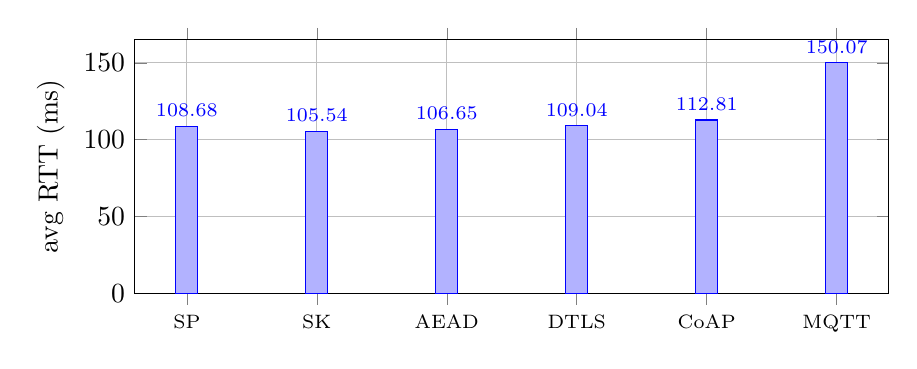
\begin{tikzpicture}
\begin{axis}[
  ybar,
  bar width=8pt,
  width=0.92\linewidth,
  height=4.8cm,
  ymin=0,
  ylabel={avg RTT (ms)},
  symbolic x coords={SP,SK,AEAD,DTLS,CoAP,MQTT},
  xtick=data,
  xticklabel style={font=\scriptsize},
  nodes near coords,
  every node near coord/.append style={font=\scriptsize},
  enlarge x limits=0.08,
  grid=major
]
\addplot coordinates {(SP,108.676) (SK,105.536) (AEAD,106.654) (DTLS,109.040) (CoAP,112.805) (MQTT,150.072)};
\end{axis}
\end{tikzpicture}

\vspace{2mm}
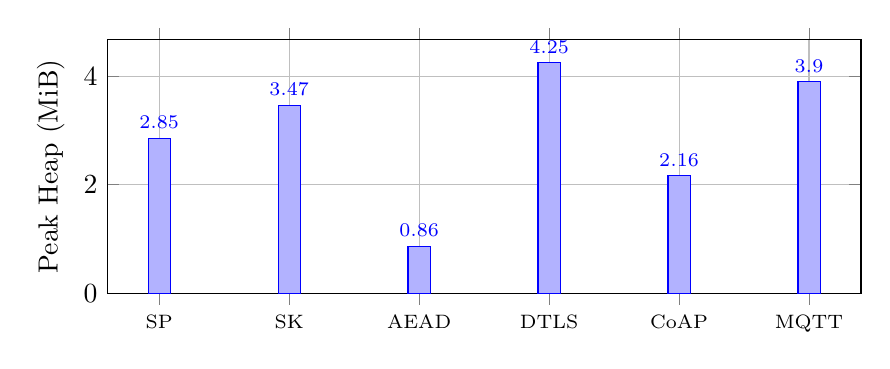
\begin{tikzpicture}
\begin{axis}[
  ybar,
  bar width=8pt,
  width=0.92\linewidth,
  height=4.8cm,
  ymin=0,
  ylabel={Peak Heap (MiB)},
  symbolic x coords={SP,SK,AEAD,DTLS,CoAP,MQTT},
  xtick=data,
  xticklabel style={font=\scriptsize},
  nodes near coords,
  every node near coord/.append style={font=\scriptsize},
  enlarge x limits=0.08,
  grid=major
]
\addplot coordinates {(SP,2.851) (SK,3.467) (AEAD,0.859) (DTLS,4.250) (CoAP,2.164) (MQTT,3.898)};
\end{axis}
\end{tikzpicture}
\caption{跨国受限网络下 RTT/峰值内存对照（SP=纯模式，SK=分包模式）}
\label{fig:c4-cross-core}
\end{figure}

\subsection{相对增益量化}
表~\ref{tab:c4-relative-gain} 给出组合数独协议相对 DTLS 与 MQTT/TLS 的增益。结果显示：组合数独协议相对 DTLS 的 RTT 优势有限（0.33\% 与 3.21\%），内存降幅分别为 32.92\% 与 18.42\%；相对 MQTT/TLS 的 RTT 优势分别为 27.58\% 与 29.68\%，内存降幅分别为 26.87\% 与 11.06\%。

\begin{table}[H]
\centering
\small
\caption{纯模式与分包模式相对 DTLS 与 MQTT/TLS 的跨国中位数增益}
\label{tab:c4-relative-gain}
\begin{tabularx}{\linewidth}{l>{\centering\arraybackslash}X>{\centering\arraybackslash}X>{\centering\arraybackslash}X>{\centering\arraybackslash}X}
\toprule
方案 & RTT 相对 DTLS & RTT 相对 MQTT & 内存相对 DTLS & 内存相对 MQTT \\
\midrule
纯组合数独 & +0.33\% & +27.58\% & +32.92\% & +26.87\% \\
6bit分包组合数独 & +3.21\% & +29.68\% & +18.42\% & +11.06\% \\
\bottomrule
\end{tabularx}
\end{table}

\subsection{开销与时延权衡}
图~\ref{fig:c4-overhead-rtt-tradeoff} 展示开销比与平均 RTT 的平面分布。纯组合数独位于高开销、同量级时延区域；6bit分包组合数独向低开销方向移动，同时保持 RTT 不劣于 DTLS，体现了两种模式在外观混淆强度与带宽效率之间的不同取舍。

\begin{figure}[!t]
\centering
\small
\begin{tikzpicture}
\begin{axis}[
  width=0.90\linewidth,
  height=6.0cm,
  xlabel={overhead ratio},
  ylabel={avg RTT (ms)},
  xmin=0.9, xmax=5.4,
  ymin=100, ymax=155,
  grid=major,
  legend style={at={(0.98,0.98)},anchor=north east,font=\scriptsize}
]
\addplot[only marks, mark=*, mark size=2.7pt] coordinates {(5.1813,108.676)};
\addlegendentry{纯组合数独}
\addplot[only marks, mark=square*, mark size=2.6pt] coordinates {(1.7389,105.536)};
\addlegendentry{6bit分包组合数独}
\addplot[only marks, mark=triangle*, mark size=2.8pt] coordinates {(1.1406,106.654)};
\addlegendentry{纯 AEAD}
\addplot[only marks, mark=diamond*, mark size=2.8pt] coordinates {(2.3279,109.040)};
\addlegendentry{DTLS}
\addplot[only marks, mark=o, mark size=2.6pt] coordinates {(1.0859,112.805)};
\addlegendentry{CoAP(UoT)}
\addplot[only marks, mark=star, mark size=3.0pt] coordinates {(2.4949,150.072)};
\addlegendentry{MQTT/TLS}
\end{axis}
\end{tikzpicture}
\caption{跨国受限网络下纯组合数独与 6bit分包的开销-时延权衡}
\label{fig:c4-overhead-rtt-tradeoff}
\end{figure}

\section{协议识别、类别恢复与主动攻击验证}
\subsection{被动侧写实验设置}
协议识别实验使用 5 轮采样，每轮 800 条消息、256B 负载、无填充。BCI 类别恢复实验构造四类负载（MI-left:80B、MI-right:82B、Blink:84B、Rest:86B），每类重复 3 轮；主报告比较三种模式：MQTT/TLS 对照、纯组合数独无填充、纯组合数独填充（20--45B 随机填充）。为补充跨协议与模式对照，本文在相同特征空间与留一法最近质心判定标准下，对 CoAP、纯 AEAD 与 6bit分包组合数独（prefer\_entropy）进行了统一复算（每协议每模式 $n=12$）。

DPI 对照实验中，组合数独 ASCII 样本由提示字节池与填充字节池按概率混合生成（提示概率 0.82），并与随机二进制样本比较可打印比例和规则分类标签。

\subsection{被动侧写结果}
侧写结果表明：协议识别准确率为 96.67\%（29/30），唯一误判来自纯组合数独与 6bit分包组合数独的一次互混；在类别恢复指标上，MQTT/TLS、CoAP/UDP、纯 AEAD 与组合数独协议无填充模式均为 1.0000，纯组合数独在 20--45B 填充模式下降至 0.1667，6bit分包组合数独（prefer\_entropy）填充模式为 0.2500。两条填充路径均显著低于无填充对照，说明填充机制可有效削弱长度序列侧写的可学习性\cite{alwhbi2024encrypted,hou2024encmalware}。

\begin{algorithm}[H]
\small
\caption{BCI 类别侧写评估：无填充为 100\%，随机填充显著降低恢复率}
\label{alg:c4-sidechannel-eval}
\KwIn{模式集合 $\mathcal{M}$，每模式样本 $\mathcal{D}_m=\{(s_i,y_i)\}$，防护策略参数 $\Pi_m$}
\KwOut{恢复率 $R_m$ 与风险等级 $L_m$}
\ForEach{$m \in \mathcal{M}$}{
  从长度序列 $s_i$ 截取 128 维窗口并提取统计特征 $x_i$\;
  采用留一法最近质心分类得到预测标签 $\hat{y}_i$\;
  $R_m \leftarrow \frac{1}{N_m}\sum_{i=1}^{N_m}\mathbf{1}(\hat{y}_i=y_i)$\;
  \eIf{$R_m \ge 0.9$}{
    $L_m \leftarrow$ 高风险（类别语义可重建）\;
  }{
    \eIf{$R_m \le 0.4$}{
      $L_m \leftarrow$ 受控风险（侧写可学习性显著下降）\;
    }{
      $L_m \leftarrow$ 中风险\;
    }
  }
}
比较 $\Pi_m=\varnothing$ 与 $\Pi_m=\text{随机填充}$ 的 $R_m$ 变化，判定防护收益\;
\end{algorithm}

从攻击语义看，被动攻击者只需观察长度序列即可恢复类别；当恢复率接近 1 时，业务类别轨迹会直接暴露，进而放大意图泄露与针对性干预风险。在 BCI-IoT 场景中，该风险将直接削弱用户隐私与控制链路安全性\cite{alwhbi2024encrypted,kapitonova2022framework,meng2024adversarial}。

协议识别召回率与 BCI 类别恢复率分别见图~\ref{fig:c4-proto-recall-extended} 和图~\ref{fig:c4-sidechannel-dpi}。

\begin{figure}[!b]
\centering
\small
\begin{tikzpicture}
\begin{axis}[
  ybar,
  bar width=9pt,
  width=0.86\linewidth,
  height=3.35cm,
  ymin=0,
  ymax=1.05,
  ylabel={协议侧写召回率},
  symbolic x coords={SP,SK,AEAD,MQTT,CoAP,DTLS},
  xtick=data,
  xticklabel style={font=\scriptsize},
  nodes near coords,
  every node near coord/.append style={font=\scriptsize},
  enlarge x limits=0.10,
  grid=major
]
\addplot coordinates {(SP,1.0) (SK,0.8) (AEAD,1.0) (MQTT,1.0) (CoAP,1.0) (DTLS,1.0)};
\end{axis}
\end{tikzpicture}
\caption{协议识别召回率对照（SP=纯模式，SK=分包模式；含 MQTT、CoAP、纯 AEAD、DTLS）}
\label{fig:c4-proto-recall-extended}
\end{figure}

进一步地，本文从协议识别混淆矩阵计算了各协议召回率（每类样本 5 轮）。图~\ref{fig:c4-proto-recall-extended} 显示，MQTT/TLS、CoAP/UDP、纯 AEAD、DTLS 与纯组合数独的召回率均为 1.0000；仅 6bit分包组合数独为 0.8000（1 次误判为纯组合数独）。这说明多类对照路线的外观特征均可被分类模型稳定学习。DPI 对照中，组合数独 ASCII 模式可打印比例为 0.9834，被归为明文样式；TLS 二进制样本为 0.3838，被归为密文二进制样式，表明外观层可改变规则式流量标签。

\begin{figure}[!t]
\centering
\small
\begin{tikzpicture}
\begin{axis}[
  ybar,
  bar width=9pt,
  width=0.90\linewidth,
  height=5.0cm,
  ymin=0, ymax=1.05,
  ylabel={类别恢复率},
  symbolic x coords={MQTT,CoAP,AEAD,SNoPad,SPad,SKPad},
  xtick=data,
  xticklabels={MQTT,CoAP,AEAD,SNoPad,SPad,SKPad},
  xticklabel style={font=\scriptsize},
  nodes near coords,
  every node near coord/.append style={font=\scriptsize},
  enlarge x limits=0.08,
  grid=major
]
\addplot coordinates {(MQTT,1.0) (CoAP,1.0) (AEAD,1.0) (SNoPad,1.0) (SPad,0.1667) (SKPad,0.25)};
\end{axis}
\end{tikzpicture}
\caption{BCI 类别恢复率对照：SNoPad=无填充，SPad=纯组合数独填充，SKPad=6bit分包填充；随机填充显著降低恢复率}
\label{fig:c4-sidechannel-dpi}
\end{figure}
\FloatBarrier

\subsection{主动攻击与 MITM 可恢复性验证}
主动攻击实验均在受控单机环境中进行：重放场景先完成一次合法握手并记录客户端发往服务端的原始握手字节，随后在第二次连接中原样重放该字节流；篡改场景在握手首个写入字节上执行单比特翻转，模拟链路中间人篡改；资源探测场景持续发送超出 $\texttt{maxProbeBytes}$ 上界的无效探测数据，观察服务端是否在握手探测阶段提前终止。对于前述三类场景，只要服务端返回的错误类型分别命中 \texttt{ErrReplayDetected}、\texttt{SuspiciousError}、\texttt{ErrAuthFailed} 或 \texttt{ErrProtocolViolation}，或在超长探测下进入可疑路径，即判定防御成功。

TLS MITM 对照实验采用另一条验证链路：攻击者先构造受控 CA 与伪造服务端证书，在客户端与真实服务端之间建立中间人代理；随后客户端按固定次序发送类别序列，代理在完成 TLS 握手后直接读取明文行并提取其中的类别字段，再将业务转发至真实服务端。若攻击者观测到的类别序列与发送序列逐项一致，则说明链路虽然采用 TLS 加密，但在终止代理点仍可恢复业务语义。表~\ref{tab:c4-security-evidence} 汇总了各攻击场景的实施动作、服务端观测与最终结果。组合数独协议在重放、篡改、资源探测三类主动攻击下均触发拒绝路径；TLS MITM 对照的恢复率为 1.0，说明攻击者可逐条恢复业务类别序列，链路加密无法消除终止代理点的业务可见性\cite{wilkens2021passivetls}。

\begin{table}[H]
\centering
\small
\caption{主动攻击与 TLS-MITM 对照：组合数独拦截重放/篡改，MITM 可恢复业务类别}
\label{tab:c4-security-evidence}
\begin{tabular}{>{\raggedright\arraybackslash}p{1.8cm}>{\raggedright\arraybackslash}p{3.5cm}>{\raggedright\arraybackslash}p{5.0cm}>{\raggedright\arraybackslash}p{1.8cm}}
\toprule
场景 & 攻击过程 & 服务端观测与成功判据 & 结果 \\
\midrule
重放攻击 & 首次握手正常完成并记录客户端握手字节；第二次连接原样重放同一字节流 & 服务端重放缓存命中，返回 \texttt{ErrReplayDetected}；命中即判定防御成功 & 成功拦截 \\
篡改攻击 & 对握手首个写入字节执行单比特翻转，再继续完成后续握手发送 & 服务端在摘要、签名或消息格式校验阶段返回 \texttt{SuspiciousError}、\texttt{ErrAuthFailed} 或 \texttt{ErrProtocolViolation}；进入拒绝路径即判定防御成功 & 成功拦截 \\
资源探测 & 向服务端连续写入远超握手探测上界的无效字节流（80KB） & 服务端在 probe 阶段因超过 \texttt{maxProbeBytes} 进入可疑路径并返回 \texttt{SuspiciousError}；提前终止即判定防御成功 & 成功拦截 \\
TLS MITM 对照 & 中间人代理使用伪造证书终止 TLS，会后逐行读取并提取 \texttt{BCI\_CLASS} 字段，再转发至真实服务端 & 将攻击者观测序列与发送序列逐项比较；恢复率接近 1 判定业务类别可恢复 & 恢复率 1.0 \\
\bottomrule
\end{tabular}
\end{table}

\subsection{Fallback 适用场景仿真}
为验证 fallback 的工程可用性，本文构造主动探测流量重定向场景：攻击侧先发送可疑握手前缀，再继续发送后续探测字节；服务端在握手阶段识别为可疑流量后，停止真实会话建立流程，并将已读前缀与后续字节转发至诱饵服务。仿真流程与结果见表 \ref{tab:c4-fallback-sim}。

\begin{table}[H]
\centering
\small
\caption{fallback 仿真：可疑握手前缀被诱饵完整接收}
\label{tab:c4-fallback-sim}
\begin{tabular}{p{2.0cm}p{4.1cm}p{4.0cm}p{2.8cm}}
\toprule
阶段 & 输入或动作 & 观测结果 & 结论 \\
\midrule
S1 可疑触发 & 发送异常握手前缀“\texttt{BAD}” & 服务端返回可疑错误并进入 fallback 路径 & 真实会话未建立 \\
\midrule
S2 连续转发 & 攻击侧继续发送“\texttt{HELLO}” & 诱饵端收到连续字节“\texttt{BADHELLO}” & 已读字节未丢失 \\
\midrule
S3 诱饵响应 & 诱饵端返回“\texttt{ACK}” & 攻击侧收到“\texttt{ACK}”响应 & 外部行为与普通服务一致 \\
\bottomrule
\end{tabular}
\end{table}

该场景表明，fallback 机制用于降低异常路径的可区分性，其作用范围限于异常流量处置。探测流量仅获得诱饵通道反馈，不返回真实协议状态。作为对照，TLS/DTLS、MQTT/TLS 与 CoAP/DTLS 路径在标准实现中通常表现为告警、断链或超时，不提供协议级已读字节回落接口（详见表 \ref{tab:c3-fallback-compare}）\cite{rfc8446,rfc9147,mqtt311,rfc7252}。

\section{对照方案风险归因与组合数独协议的工程权衡}
结合协议机理与实证结果，第 4 章的对比结论可置于“安全属性与工程成本同步分配”的分析框架中解释。BCI 场景需要将隐私与安全要求前置到系统设计阶段\cite{kapitonova2022framework}，IoT 安全方案也必须兼顾敏感数据保护、资源约束与部署适配\cite{trabelsi2023iotaccess}。

需要强调的是，本文方案的价值在于把握手认证、会话加密与外观抗侧写放入同一协议状态机，并为每一项安全属性支付明确成本：协议引入数独编码、可逆外观映射和随机填充后，确实增加了编码复杂度与线长/带宽开销；但长度序列、可打印比例和 DPI 标签不再与业务类别保持简单对应。若威胁模型仅关注端到端机密性与完整性，DTLS/MQTT-TLS 的成熟生态仍更合适；当攻击者能够长期观察链路并利用长度、时序或 DPI 标签实施侧写时，组合数独外观层提供了主流安全隧道之外的额外防护维度。

\begin{itemize}
  \item \textbf{CoAP（UDP）}：协议语义建立在 UDP 之上\cite{rfc7252}，但在跨国受限链路中需通过 UoT 中继，原生 UDP 部署优势难以直接发挥。
  \item \textbf{DTLS}：具备标准化握手与会话保护\cite{rfc9147}，但在受限公网常依赖中继与代理，运维信任范围扩大。
  \item \textbf{MQTT/TLS}：生态成熟、工程复用高\cite{mqtt311,rfc8446,zheng2023mqtttamarin}，但长度与时序特征仍可被侧写模型稳定利用\cite{alwhbi2024encrypted,hou2024encmalware}。
  \item \textbf{纯 AEAD}：记录层机密性与完整性明确\cite{rfc5116}，但缺乏独立握手认证与新鲜性语义，抗重放能力依赖额外状态机。
  \item \textbf{组合数独协议}：通过握手防护、外观调控与资源控制实现联合优化；纯模式偏重混淆能力，分包模式偏重带宽效率。
\end{itemize}

因此，组合数独协议在 BCI-IoT 场景下可视为兼顾安全语义、资源约束与外观调控能力的可部署方案：相较纯 AEAD，安全语义更完整；相较 MQTT/DTLS，在被动侧写威胁下具有更强的外观对抗能力；代价是纯模式路径带宽开销较高、实现复杂度和标准化生态仍需扩展（见表~\ref{tab:c4-cross-region-main}、图~\ref{fig:c4-sidechannel-dpi}、表~\ref{tab:c4-security-evidence}）。

\section{有效性威胁与适用条件}
本文结果在下列条件内成立。
\begin{itemize}
  \item \textbf{外部有效性}：跨国实验基于单个公网节点，未覆盖全部地区与运营商网络。
  \item \textbf{统计有效性}：跨国重复次数为 3，适合趋势判断，不用于细粒度显著性检验。
  \item \textbf{模型有效性}：侧写模型以特征工程为主，未覆盖大规模深度时序模型上界。
  \item \textbf{原型有效性}：结论对应本文所实现的协议原型，若迁移到其他语言或实现框架，仍需重新评估。
\end{itemize}

\section{本章小结}
本章建立了实验设计、指标算法、攻击判定与结果解释的一致性链路。结果显示：在跨国受限网络中，组合数独协议的 RTT 与主流协议处于同量级，数据面内存低于 DTLS 与 MQTT/TLS；在安全与对抗方面，组合数独协议可稳定拦截重放与篡改，填充机制可显著降低类别侧写恢复率。综合来看，组合数独协议具备可量化、可复核、可部署的应用可行性。

\chapter{全文总结与展望}

\section{全文总结}
本文面向 BCI-IoT 场景的“敏感数据 + 实时性 + 资源受限”约束，设计并实现了 IoT\_BCI-Sudoku 安全通信增强协议。协议在身份认证握手与会话 AEAD 加密的基础上，引入 Sudoku 外观层（映射编码、随机填充与布局轮转），并提供抗重放、异常回落与可复现评测工具链。通过与纯 AEAD、DTLS、MQTT 与 CoAP/UDP 等基线协议的对比实验，本文给出在带宽开销、时延、内存与外观指标上的量化结果，并讨论了安全性、效率与抗侧写能力之间的工程权衡。

\section{后续工作展望}
结合当前实现与评测进度，后续可从以下方向进一步完善：
\begin{itemize}
  \item \textbf{端侧资源上限参数化}：为不同设备规格提供默认配置与上限保护（连接状态、缓冲区、回落策略阈值）。
  \item \textbf{更系统的安全验证}：补充 fuzz 测试覆盖握手/解码/状态机边界，并在 CI 中固定运行静态检查与竞态检测。
  \item \textbf{更贴近真实网络的极端场景}：增加可复现的高抖动/丢包/拥塞场景测试脚本与统计口径，用于评估鲁棒性与性能波动。
  \item \textbf{密钥生命周期管理}：支持证书吊销/轮换、会话密钥更新与多设备部署下的集中化管理。
  \item \textbf{进一步降低开销}：在不牺牲安全语义的前提下，持续优化内存分配、减少写调用次数，并探索更高效的 padding 策略。
\end{itemize}



\thesisacknowledgement
本论文在导师邢建川副教授的悉心指导下完成。导师在选题论证、研究方法、实验设计与论文写作等环节给予了系统而严谨的指导，在此谨致以诚挚谢意。

感谢学院提供的实验环境与资源保障，使本研究能够完成从代码实现到实证评估的完整闭环。

感谢父母和家人在本科阶段长期的理解、鼓励与支持。你们给予的信任与包容，是我持续投入学习和完成毕业设计的重要动力。

\thesisappendix

\chapter{复现实验命令清单}
\section{编译与自检}
在仓库根目录执行：
\begin{verbatim}
go test ./...
go test -race ./...
\end{verbatim}

\section{运行协议示例（回环）}
\begin{verbatim}
go run ./cmd/iotbci -c configs/dev_server_stream.json -timeout 30s
go run ./cmd/iotbci -c configs/dev_client_stream.json -timeout 30s
\end{verbatim}

\section{生成 bench / evidence / dashboard}
\begin{verbatim}
go run ./cmd/iotbci-bench -messages 1000 -size 256 -timeout 30s -out bench.json
go run ./cmd/iotbci-evidence -out_dir evidence_out -messages 200 -size 256 -timeout 30s
go run ./cmd/iotbci-attack -timeout 10s -out attack_report.json
go run ./cmd/iotbci-dashboard -bench bench.json -evidence evidence_out/evidence.json -attack attack_report.json -out_dir dashboard_out
\end{verbatim}

\section{生成 LaTeX 图表与表格}
\begin{verbatim}
go run ./cmd/iotbci-texgen -bench bench.json -evidence evidence_out/evidence.json -out_dir tex/generated
\end{verbatim}



\thesisbibliography{reference}

\end{document}
